\part{Chalcogen bonding at oxygen}
\begin{refsection}

\chapter{Experimental evidence of Chalcogen bonding at oxygen.}

This chapter was published in Chem. Commun., 13 Feb 2020\autocite{Fellowes2020}. \footnote{Compound numbering, section titles, and terminology have been updated to fit this thesis.}

\section{Abstract}
An \emph{o}-nitro-O-aryl oxime was observed to exhibit a short O$\cdots$O contact, which exhibited characteristics consistent with a chalcogen bond.
The \ce{O-N} bond length of the oxime was appreciably longer than the expected value, and
NBO calculations indicated the presence of a n(O)$\rightarrow \sigma^{\star}$(\ce{O-N}) orbital delocalisation.
Topological analysis of the experimental electron density of two analogues shows the presence of a bond path between the two oxygen atoms, with $\rho(r)$ and $\nabla^{2}\rho(r)$ values consistent with an electrostatic interaction.
Finally, electrostatic potential calculations indicate the presence of a $\sigma$-hole, the ``smoking gun'' indicating a Ch-bond.
These results are unusual as oxygen is not typically considered to be a Ch-bond donor, especially in unactivated systems such as oximes.

\section{Introduction}
Chalcogen bonding (Ch-bonding) is a weak interaction of the broader family of $\sigma$-hole interactions, in which a chalcogen atom adopts some electrophilic character, allowing it to form a stabilised complex with a Lewis base.
Much work has been directed towards applying Ch-bonding principles to fields such as supramolecular engineering, catalysis, and anion sensing.\autocite{Riwar2018,Mahmudov2017,Wonner2019,Ho2016,Kremer2016,Benz2017a}
Typically only the heavier chalcogen atoms form Ch-bonds (tellurium, selenium or sulfur, the latter having particular relevance to protein folding).\autocite{Iwaoka2012}
The reason for this is that the electron cloud of the chalcogen must be distorted by an electron withdrawing substituent in order to form the electrophilic $\sigma$-hole.
The larger and more polarisable the chalcogen atom, the more electrophilic the $\sigma$-hole, and the stronger the Ch-bond.\autocite{Murray2008}

Oxygen, as the second most electronegative element with its extremely low polarisability, is not considered to be a strong Ch-bond donor, although recent theoretical studies indicate that it can form a $\sigma$-hole in species such as \ce{OF2} and \ce{FNO3}.\autocite{Varadwaj2019a,Varadwaj2019}
We report here a compound which appears to contain an intramolecular O$\cdots$O Ch-bond, which was synthesised and crystallised as part of an investigation into the Beckmann rearrangement.\autocite{Yeoh2012}

\begin{figure}
\centering
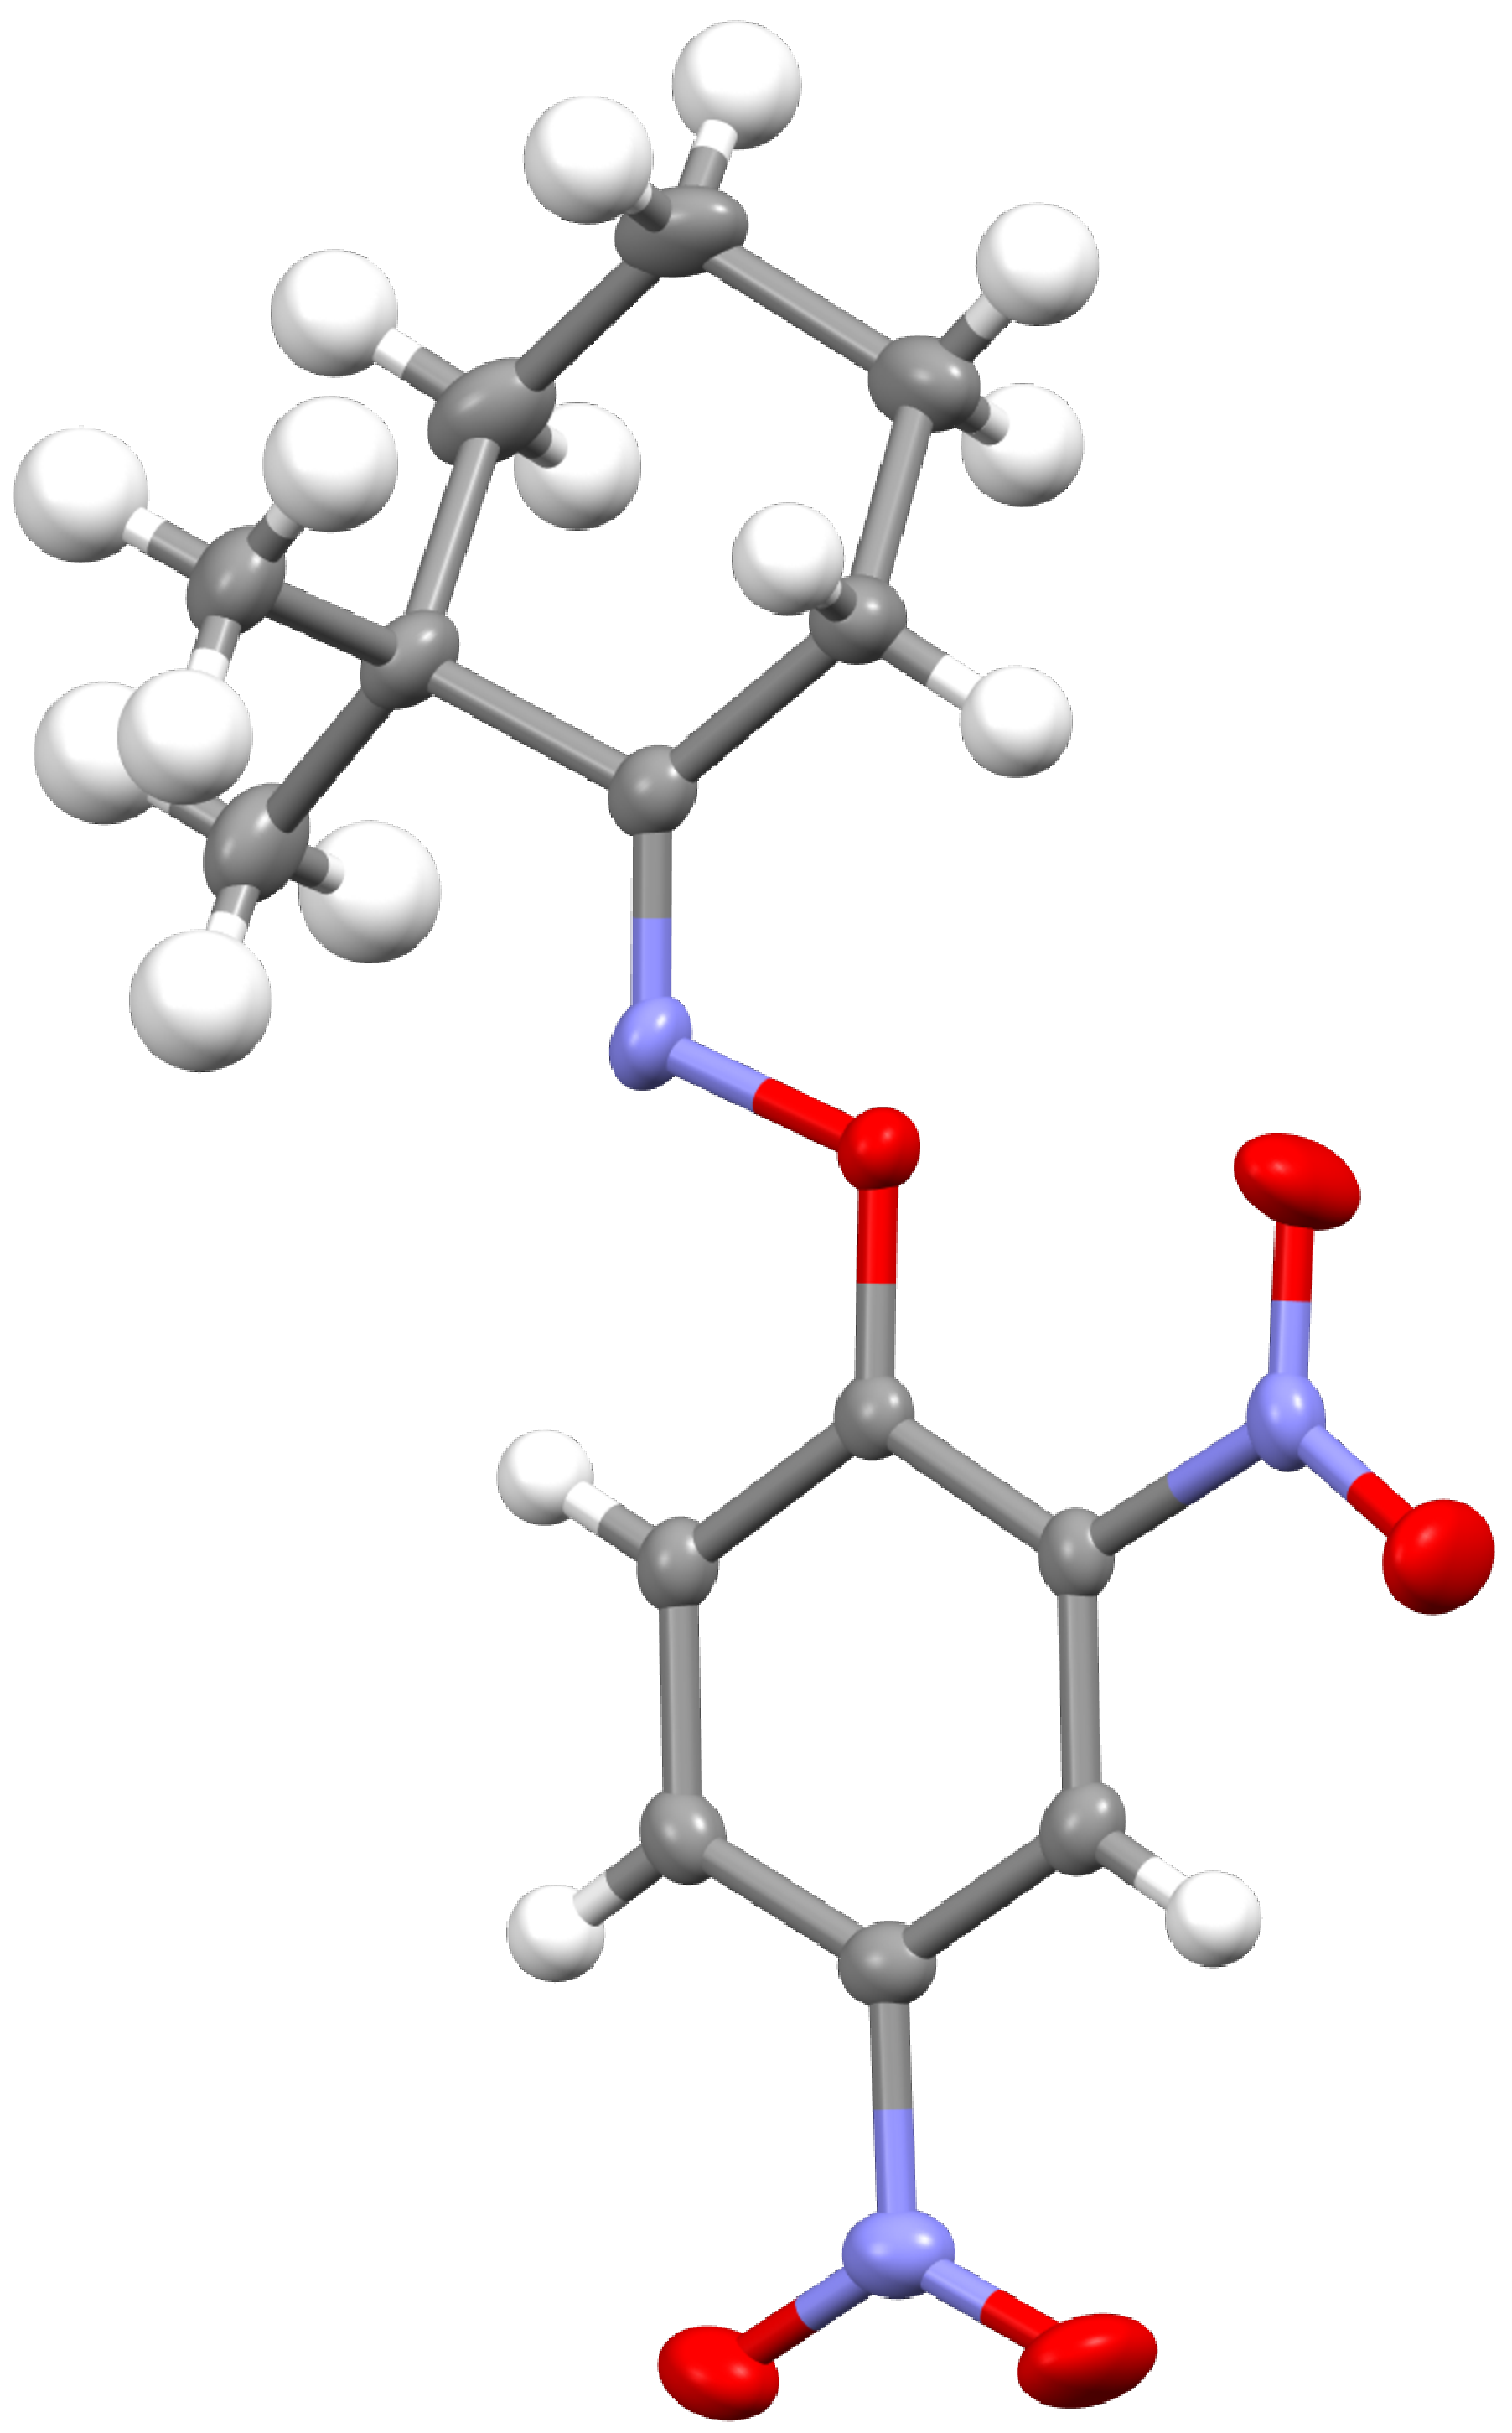
\includegraphics[width=3cm]{Figures/dimethylcyclohexanone-oxime-dnp-xray.pdf}
\hspace{0.5cm}
\replacecmpd{dimethylcyclohexanone-oxime-dnp}
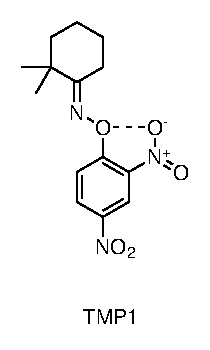
\includegraphics[scale=0.74]{Figures/dimethylcyclohexanone-oxime-dnp.eps}
\caption{Oxime \refcmpd{dimethylcyclohexanone-oxime-dnp} displays a close O$\cdots$O contact, which has characteristics consistent with a Ch-bond.}
\label{fig:dimethylcyclohexanone-oxime-dn}
\end{figure}

\section{Results and Discussion}
The compound \cmpd{dimethylcyclohexanone-oxime-dnp} is an \emph{o}-nitro-O-aryl oxime, in which the nitro group constitutes the Ch-bond acceptor, and the oxime is the Ch-bond donor.
Although the coplanar geometry of the oxime and nitro groups is expected on the grounds of favourable conjugation of these groups into the aromatic ring, there are a number of signs that suggest that there is an additional stabilising interaction between the groups, namely, the Ch-bond.

\subsection{Structural effects attributable to the Ch-bond}
\begin{table}
\centering
\caption[Selected geometric parameters of oximes \refcmpd{dimethylcyclohexanone-oxime-dnp}, \refcmpd{cyclohexanone-oxime-dnp} and \refcmpd{acetone-oxime-dnp}.]{Selected geometric parameters of oximes \refcmpd{dimethylcyclohexanone-oxime-dnp}, \refcmpd{cyclohexanone-oxime-dnp} and \refcmpd{acetone-oxime-dnp}. The two geometries in the asymmetric unit of \refcmpd{cyclohexanone-oxime-dnp} are indicated as \refcmpd{cyclohexanone-oxime-dnp}a and \refcmpd{cyclohexanone-oxime-dnp}b.}
\small
\begin{tabular}{llllll}\toprule
	Compound & r(\ce{O1}$\cdots$\ce{O2}) & r(\ce{N1O1}) & r(\ce{N2O2}) & $\angle$(\ce{O2}$\cdots$\ce{O1N1}) & $\angle$(\ce{C1C2N2O2})\\
	& \AA & \AA & \AA & $^\circ$ & $^\circ$ \\\midrule
	\cmpd{dimethylcyclohexanone-oxime-dnp} 	& 2.619(2)	& 1.489(2)	& 1.208(2)	& 161.80(8)	& -3.5(2)	\\
	\cmpd{cyclohexanone-oxime-dnp}a & 2.5423(8) & 1.4556(7) & 1.2264(9) & 160.56(5) & -0.7(1)	\\
	\cmpd{cyclohexanone-oxime-dnp}b & 2.5522(8) & 1.4522(7) & 1.223(1) 	& 160.29(4) & -0.2(1)	\\
	\cmpd{acetone-oxime-dnp} 	& 2.6390(8) & 1.4480(7) & 1.2266(8) & 148.60(4) & -30.94(8)	\\\bottomrule
\end{tabular}
\end{table}

Firstly, bond lengths measured from the crystal structure deviate somewhat from expected values.
The O$\cdots$O Ch-bond distance was measured to be 2.619(2)~\AA, which is well within the van der Waals radii of two oxygen atoms (3.04~\AA).\autocite{Bondi1964}
The \ce{O-N} bond of the oxime is also lengthened appreciably.
Comparisons with other O-aryl oximes are convoluted by the significant effect of the electronic properties of the phenyl ring on the oxime bond length.
However, an expected value can be calculated using the acidity of the corresponding 2,4-dinitro phenol (p$K_{\mathrm{a}}$ = 5.91) and the structural correlation given in equation \cref{eqn:scp}.\autocite{Yeoh2012,Socrates1970}

\begin{equation}
	r_{\mathrm{N-OR}} (\text{\AA}) = 1.467 - (3.20\times10^{-3}) \times \mathrm{p}K_{\mathrm{a}}(\mathrm{ROH})
	\label{eqn:scp}
\end{equation}

This gives an expected bond length of 1.448~\AA~versus the measured bond length 1.489(2)~\AA\ ($\Delta = 0.041$~\AA~$= 13.7\sigma$).

This is consistent with the charge transfer model of Ch-bonding, as the lone pair of the nitro oxygen donor is delocalised into the $\sigma^{\star}$\ce{(O-N)} antibonding orbital, leading to a weakening and lengthening of this bond.\autocite{Reed1988}

\subsection{NBO calculations}
Secondly, DFT calculations were carried out on the solid phase geometry of \cmpd{dimethylcyclohexanone-oxime-dnp} in order to ascertain the nature of the O$\cdots$O close contact within the NBO (Natural Bond Orbital) and QTAIM (Quantum Theory of Atoms In Molecules) frameworks.\autocite{Bader1991,NBO7}
The two frameworks are complementary descriptions of bonding within molecules.
The calculations were performed at the M06-2X/aug-cc-pVQZ level as implemented in the Gaussian16 suite.\autocite{gaussian16,Zhao2008,Woon1995}
This has been shown to give accurate densities for Ch-bonded complexes.\autocite{Kim2019}

It is customary to optimise structures so they are at a gas-phase minimum, ensuring that any derived energies, vibrational modes, and other quantities are reliable.
In this case, however, we were unable to locate a minimum corresponding to the crystal geometry; the nitro group was forced out of the plane of the aryl ring, disrupting the requisite Ch-bond geometry.
We note that the potential energy surface of this torsion is quite shallow, so the lack of a satisfactory minimum is likely due to the absence of crystal packing.
Regardless, a thorough investigation was considered to be outside of the scope of this preliminary study, therefore solid phase geometries were used instead, with the caveat that certain quantities are likely to be unreliable.

The NBO calculations revealed the presence of a n(O)$\rightarrow \sigma^{\star}$(\ce{O-N}) orbital delocalisation, which is one criterion by which a Ch-bond can be defined.\autocite{Pascoe2017}
As the geometry at which the NBO analysis was performed was not a gas phase minimum, orbital energies are inaccurate, and so the usual estimate of the strength of a delocalisation ($E^2$) should not be used.
We instead measure the magnitude of the delocalisation using the off-diagonal element of the Fock matrix $F(i,j)$, from which the energy $E^2$ is calculated using equation \cref{eqn:fock}.

\begin{equation}
	E^2 = q_i \frac{F(i,j)^2}{\epsilon_j - \epsilon_i}
	\label{eqn:fock}
\end{equation}

The value of $F(i,j)$ for the n(O)$\rightarrow \sigma^{\star}$(\ce{O-N}) orbital delocalisation in \cmpd{dimethylcyclohexanone-oxime-dnp} is 0.023~a.u., indicating a small delocalisation.

\subsection{QTAIM analysis of electron density}
Bader's Quantum Theory of Atoms In Molecules (QTAIM) describes bonding in terms of the observable quantity of electron density and its topology.
We analysed the DFT density of oxime \cmpd{dimethylcyclohexanone-oxime-dnp}, which revealed the presence of a bond path between the two oxygen atoms.
Bond paths are associated with bond critical points (bcps), where the gradient vector of the electron density is zero.

The values of both the electron density $\rho(r)$ and the Laplacian of the electron density $\nabla^{2}\rho(r)$ at the bcp are diagnostic of certain types of bonds.
Bcps with a small $\rho(r)$ and positive $\nabla^{2}\rho(r)$ (indicating local depletion of electron density at the bcp) are characteristic of ionic bonds or purely electrostatic interactions.
The values of $\rho(r)$ and $\nabla^{2}\rho(r)$ respectively are 0.0161 and +0.0790 (in a.u.), suggesting this is primarily a closed shell electrostatic interaction, and that the NBO delocalisation, although present, is secondary.

These observations piqued our interest in the potential for Ch-bonding at oxygen, so we decided to extend our investigation to verify that this interaction was not simply a quirk of the initial oxime.

\subsection{CSD search for similar structures}
\begin{figure}
\centering
	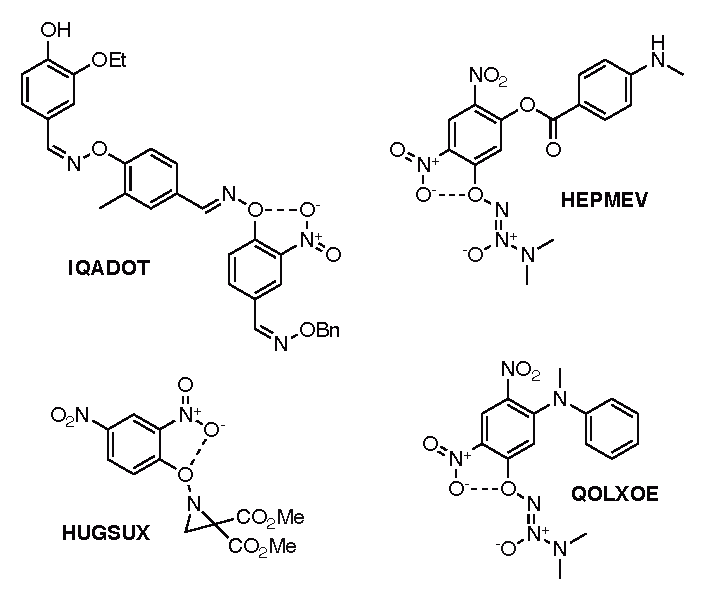
\includegraphics[scale=0.74]{Figures/csd-search-1.eps}
	\caption{Structures of CSD matches for the \emph{o}-nitro-O-aryl oxime motif.}
	\label{fig:csd}
\end{figure}

\begin{table}
\centering
\caption{Selected geometric parameters of structures HEPMEV, HUGSUX, QOLXOE, and IQADOT}
\label{tab:csd}
\small
\begin{tabular}{llllll}\toprule
	Compound & r(\ce{O1}$\cdots$\ce{O2}) & r(\ce{N1-O1}) & r(\ce{N2-O2}) & $\angle$(\ce{O2}$\cdots$\ce{O1-N1}) & $\angle$(\ce{C1-C2-N2-O2})\\
	& \AA & \AA & \AA & $^\circ$ & $^\circ$ \\\midrule
	\textbf{HEPMEV} & 2.554(5)	& 1.426(4)& 1.222(4)	& 161.2(2)	& -15.4(6)	\\
	\textbf{HUGSUX} & 2.563(2) 	& 1.461(2) & 1.220(2) 	& 158.4(1) 	& 20.8(2)	\\
	\textbf{QOLXOE}	& 2.557(4) 	& 1.419(4) & 1.216(5) 	& 158.7(2) 	& -10.9(6) 	\\
	\textbf{IQADOT}a& 2.532(2) 	& 1.445(2) & 1.207(3) 	& 154.4(1) 	& -9.2(3) 	\\
	\textbf{IQADOT}b& ---	 	& 1.433(2) & ---		& ---		& ---	 	\\\bottomrule
\end{tabular}
\end{table}

A search of the Cambridge Structural Database for \emph{o}-nitro-O-aryl oximes afforded several results.\autocite{CSD}
Structures HEPMEV, HUGSUX, and QOLXOE all contained similar motifs to \cmpd{dimethylcyclohexanone-oxime-dnp}, with a nitro group approximately coplanar with an \emph{ortho} oxime or oxime-like group.\autocite{Saavedra2001,Kostyanovsky2002,Saavedra2006a}
Structure IQADOT was particularly interesting, as it contains two electronically similar oximes, only one of which has an \emph{ortho} nitro group.\autocite{Renaudet2003}
The difference in bond lengths between them is significant (1.445(2)~\AA~versus 1.433(2)~\AA, $\Delta = 0.012$~\AA~$= 6\sigma$), and the same trend is observed as in \cmpd{dimethylcyclohexanone-oxime-dnp}.
Relevant structural parameters are given in table \cref{tab:csd}.

\subsection{Analysis of analogues and determination of experimental electron density}
Two analogues of oxime \cmpd{dimethylcyclohexanone-oxime-dnp} (\cmpd{cyclohexanone-oxime-dnp} and \cmpd{acetone-oxime-dnp}, figure \cref{fig:analogues}) were prepared, forming crystals which gave data of sufficient quality for multipole refinement, allowing us to analyse the experimental electron density as opposed to the calculated DFT density.\autocite{Hansen1978}
This refinement was performed using the MoProSuite software package.\autocite{Jelsch2005}
\cmpd{cyclohexanone-oxime-dnp} crystallised in a similar coplanar geometry to \cmpd{dimethylcyclohexanone-oxime-dnp}, exhibiting a Ch-bond\footnote[1]{The asymmetric unit contained two molecules, however both had similar geometries, and in the interests of simplicity values for only one molecule are presented.}, while \cmpd{acetone-oxime-dnp} displayed a torsion of the nitro group, disrupting the requisite geometry.
This torsion can be attributed to crystal packing forces (taken to be worth 0.5--2~kcal/mol) disrupting this extremely weak interaction.\autocite{Dunitz2009}

\begin{figure}
	\centering
	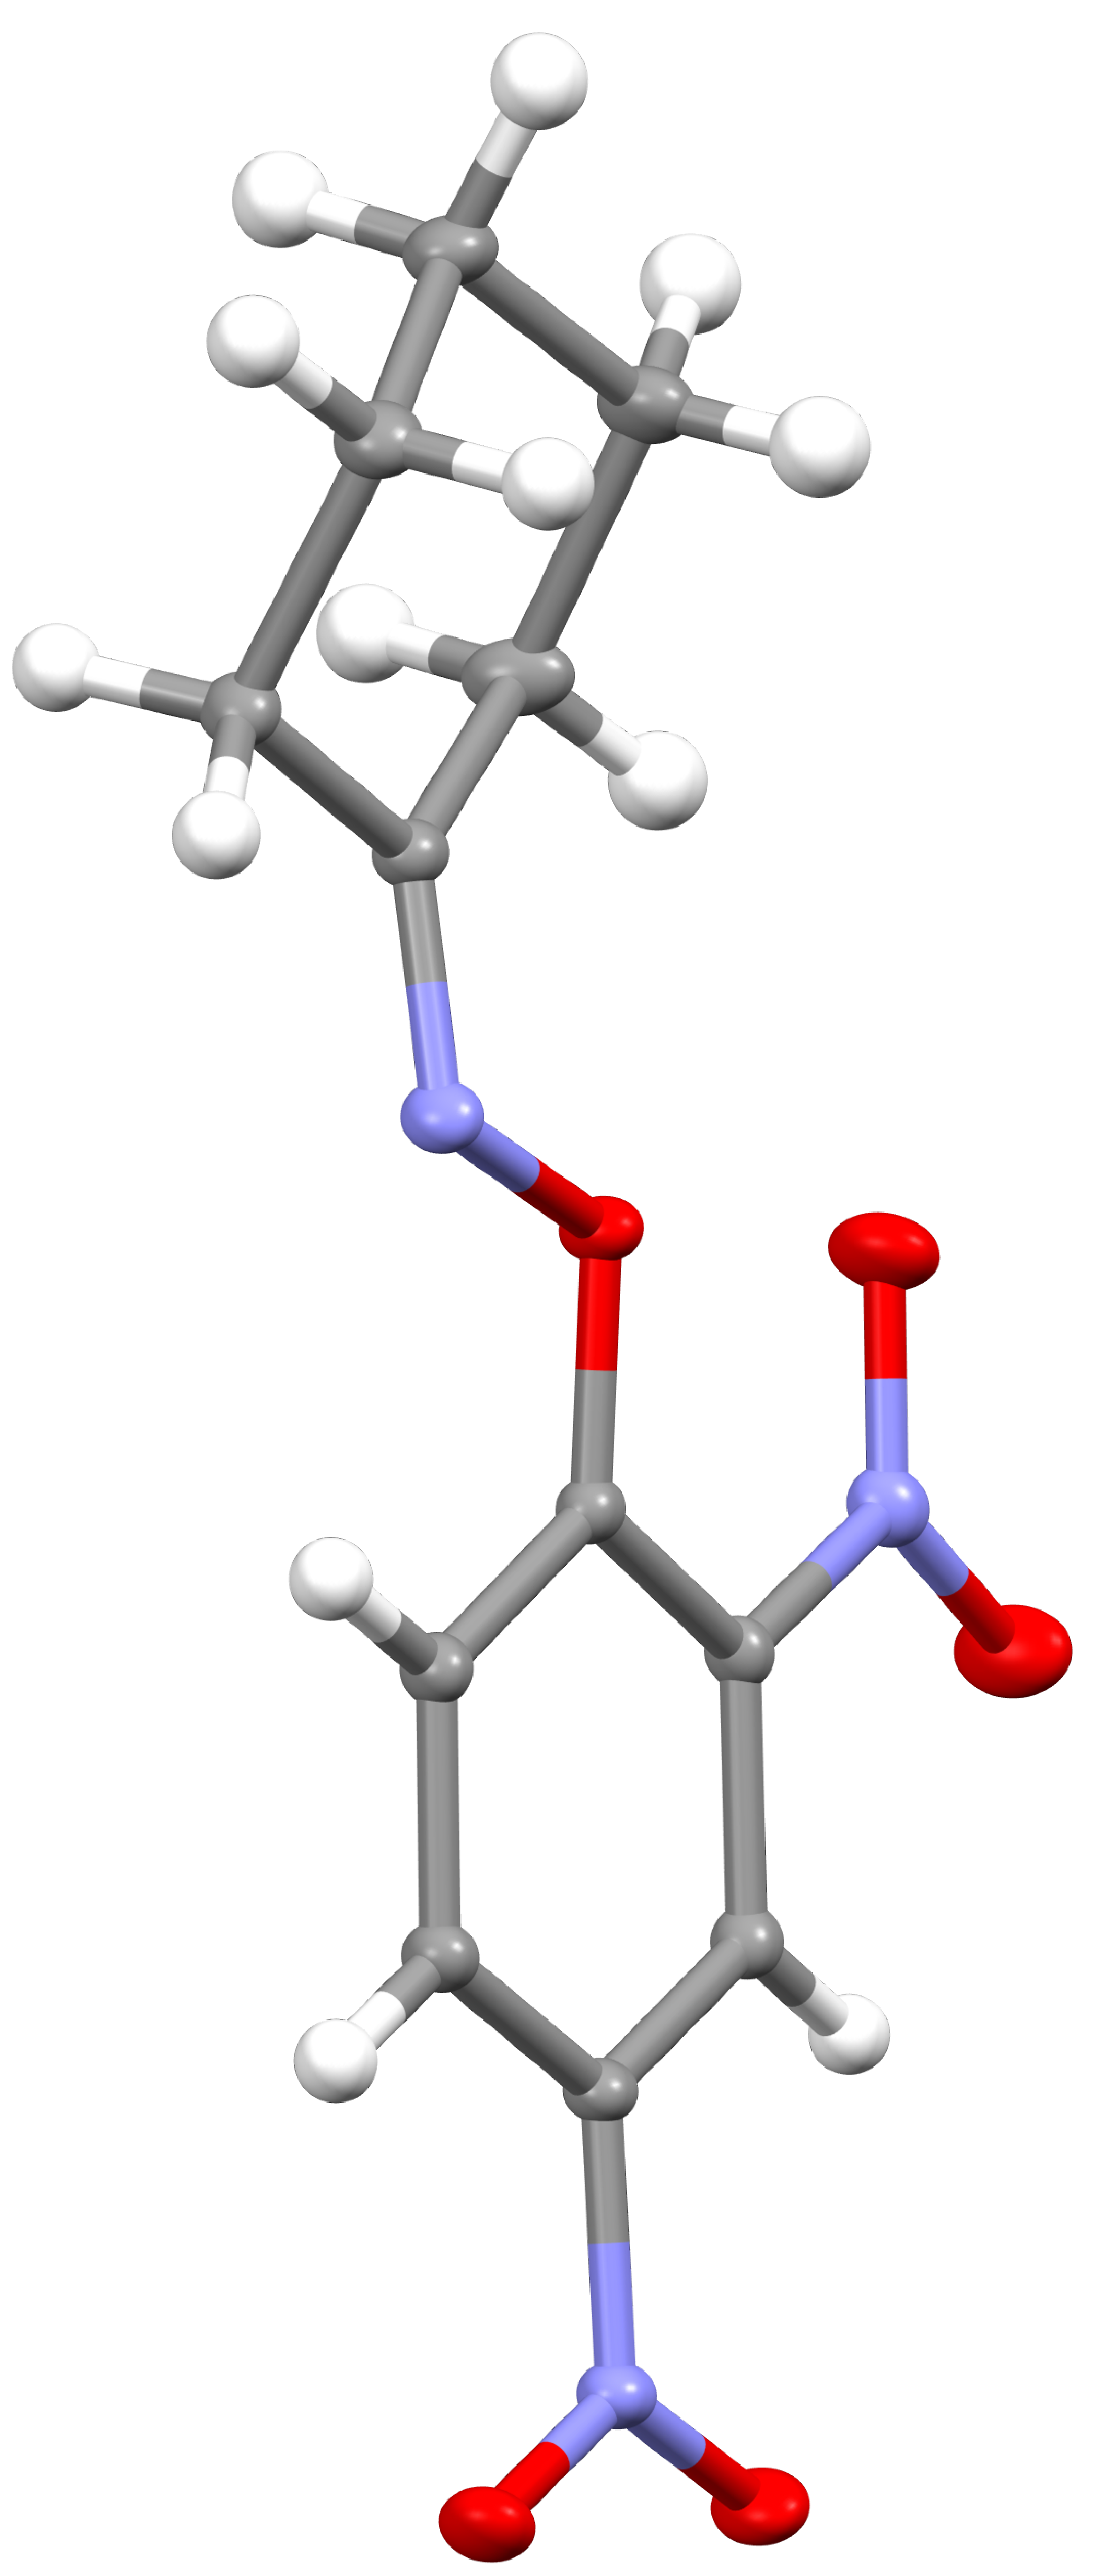
\includegraphics[width=2cm]{Figures/cyclohexanone-oxime-dnp-xray.pdf}
	\replacecmpd{cyclohexanone-oxime-dnp}
	\replacecmpd{acetone-oxime-dnp}
	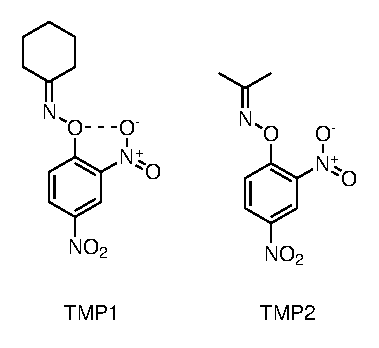
\includegraphics[scale=0.74]{Figures/oximes.eps}
	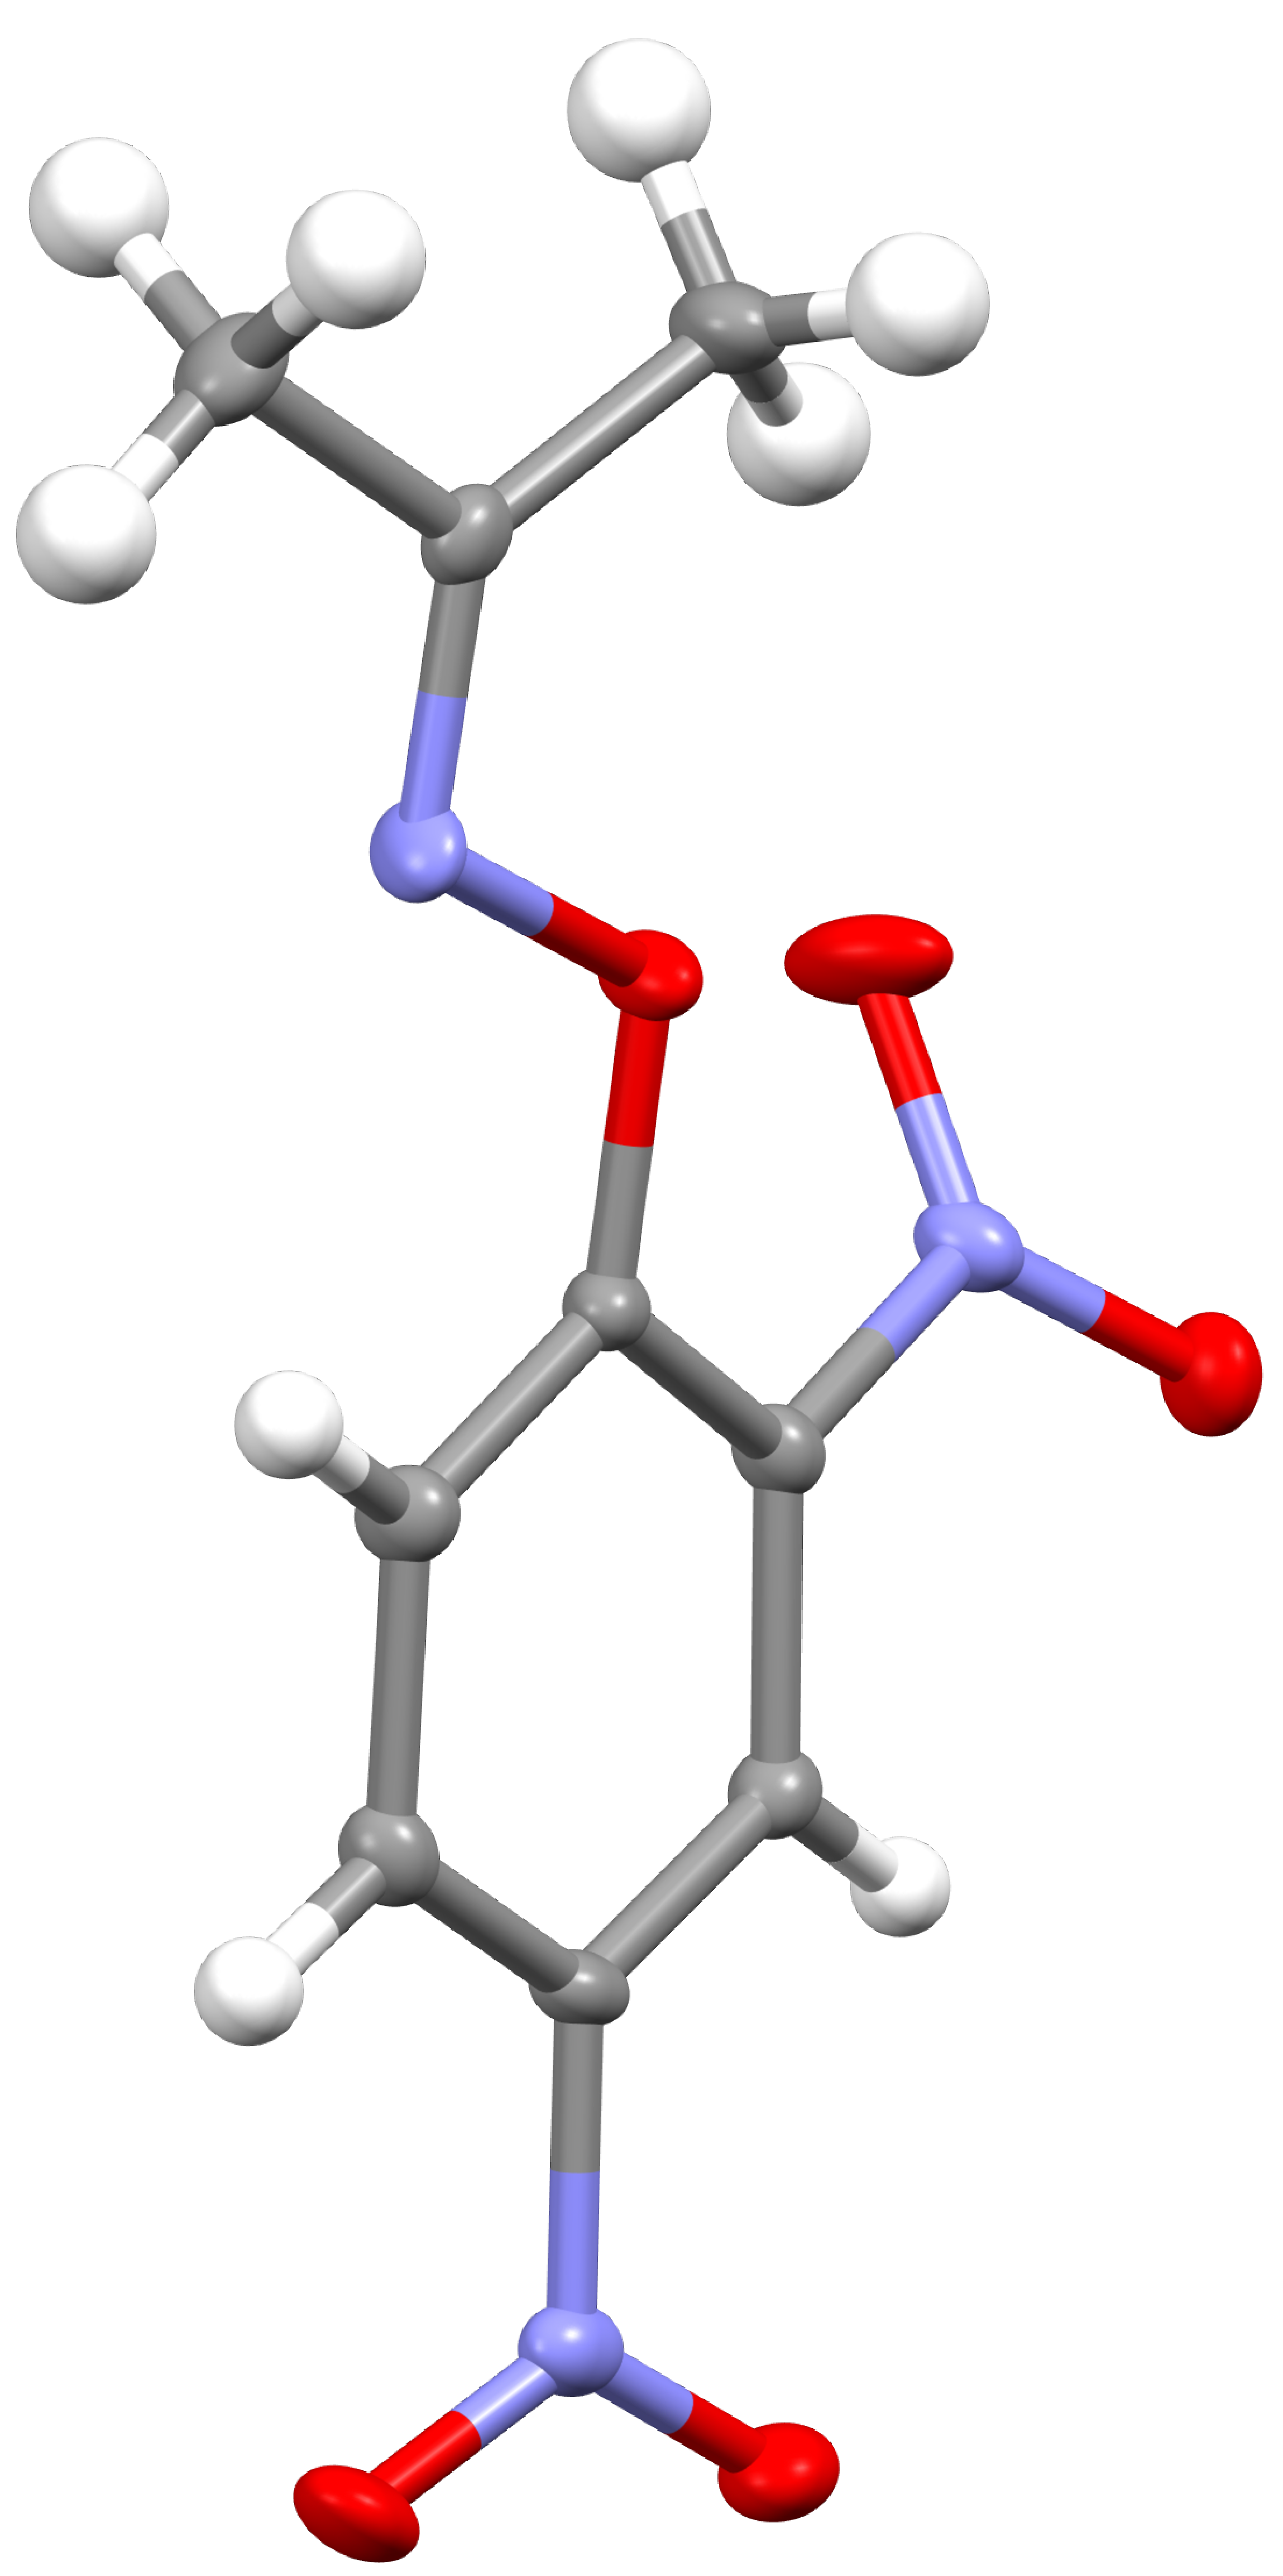
\includegraphics[width=2cm]{Figures/acetone-oxime-dnp-xray.pdf}
	\caption{Oxime \refcmpd{cyclohexanone-oxime-dnp} adopts a similar conformation to \refcmpd{dimethylcyclohexanone-oxime-dnp}, while the nitro group of \refcmpd{acetone-oxime-dnp} is twisted, leading to poor alignment with the oxime.}
	\label{fig:analogues}
\end{figure}

The oxime bond lengths differ significantly between \cmpd{cyclohexanone-oxime-dnp} and \cmpd{acetone-oxime-dnp} (1.4556(7)--1.4522(7) versus 1.4480(7)~\AA, $\Delta = 0.0042~\text{\AA} = 6\sigma$), supporting the suggestion that the n(O)$\rightarrow \sigma^{\star}$(\ce{O-N}) orbital delocalisation plays a role in these Ch-bonds.
NBO analysis of these geometries confirmed this, with $F(i,j)$ values of 0.026~a.u. for \cmpd{cyclohexanone-oxime-dnp}, and an absence of any delocalisation in \cmpd{acetone-oxime-dnp}.

QTAIM analysis of the experimental density revealed the presence of a bond path and bcp in \cmpd{cyclohexanone-oxime-dnp} but not in \cmpd{acetone-oxime-dnp}, showing that there is indeed an interaction present when the geometry allows.
In \cmpd{cyclohexanone-oxime-dnp}, the values of $\rho(r)$ and $\nabla^{2}\rho(r)$ respectively are 0.018 and +0.094 (in a.u.), which agree well with the DFT values calculated for \cmpd{dimethylcyclohexanone-oxime-dnp}, and are consistent with a closed-shell origin for the interaction (figure \cref{fig:lapl}).

\begin{figure}
	\centering
	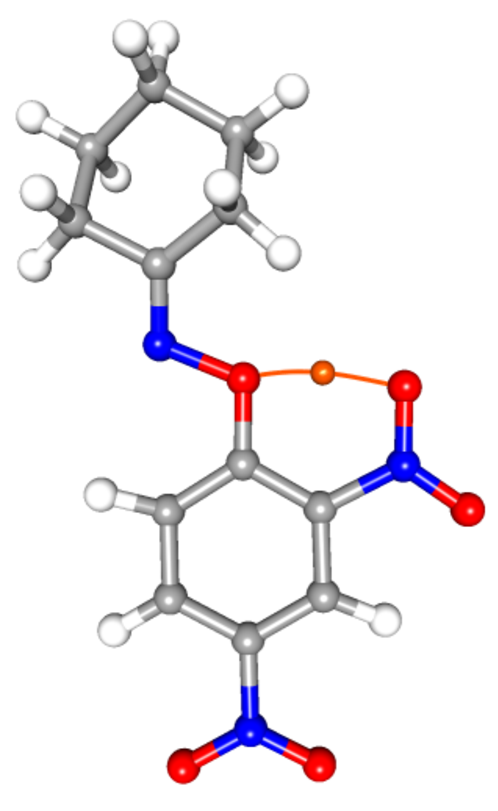
\includegraphics[width=0.3\columnwidth]{Figures/cyclohexanone-oxime-dnp-bcp.pdf}

	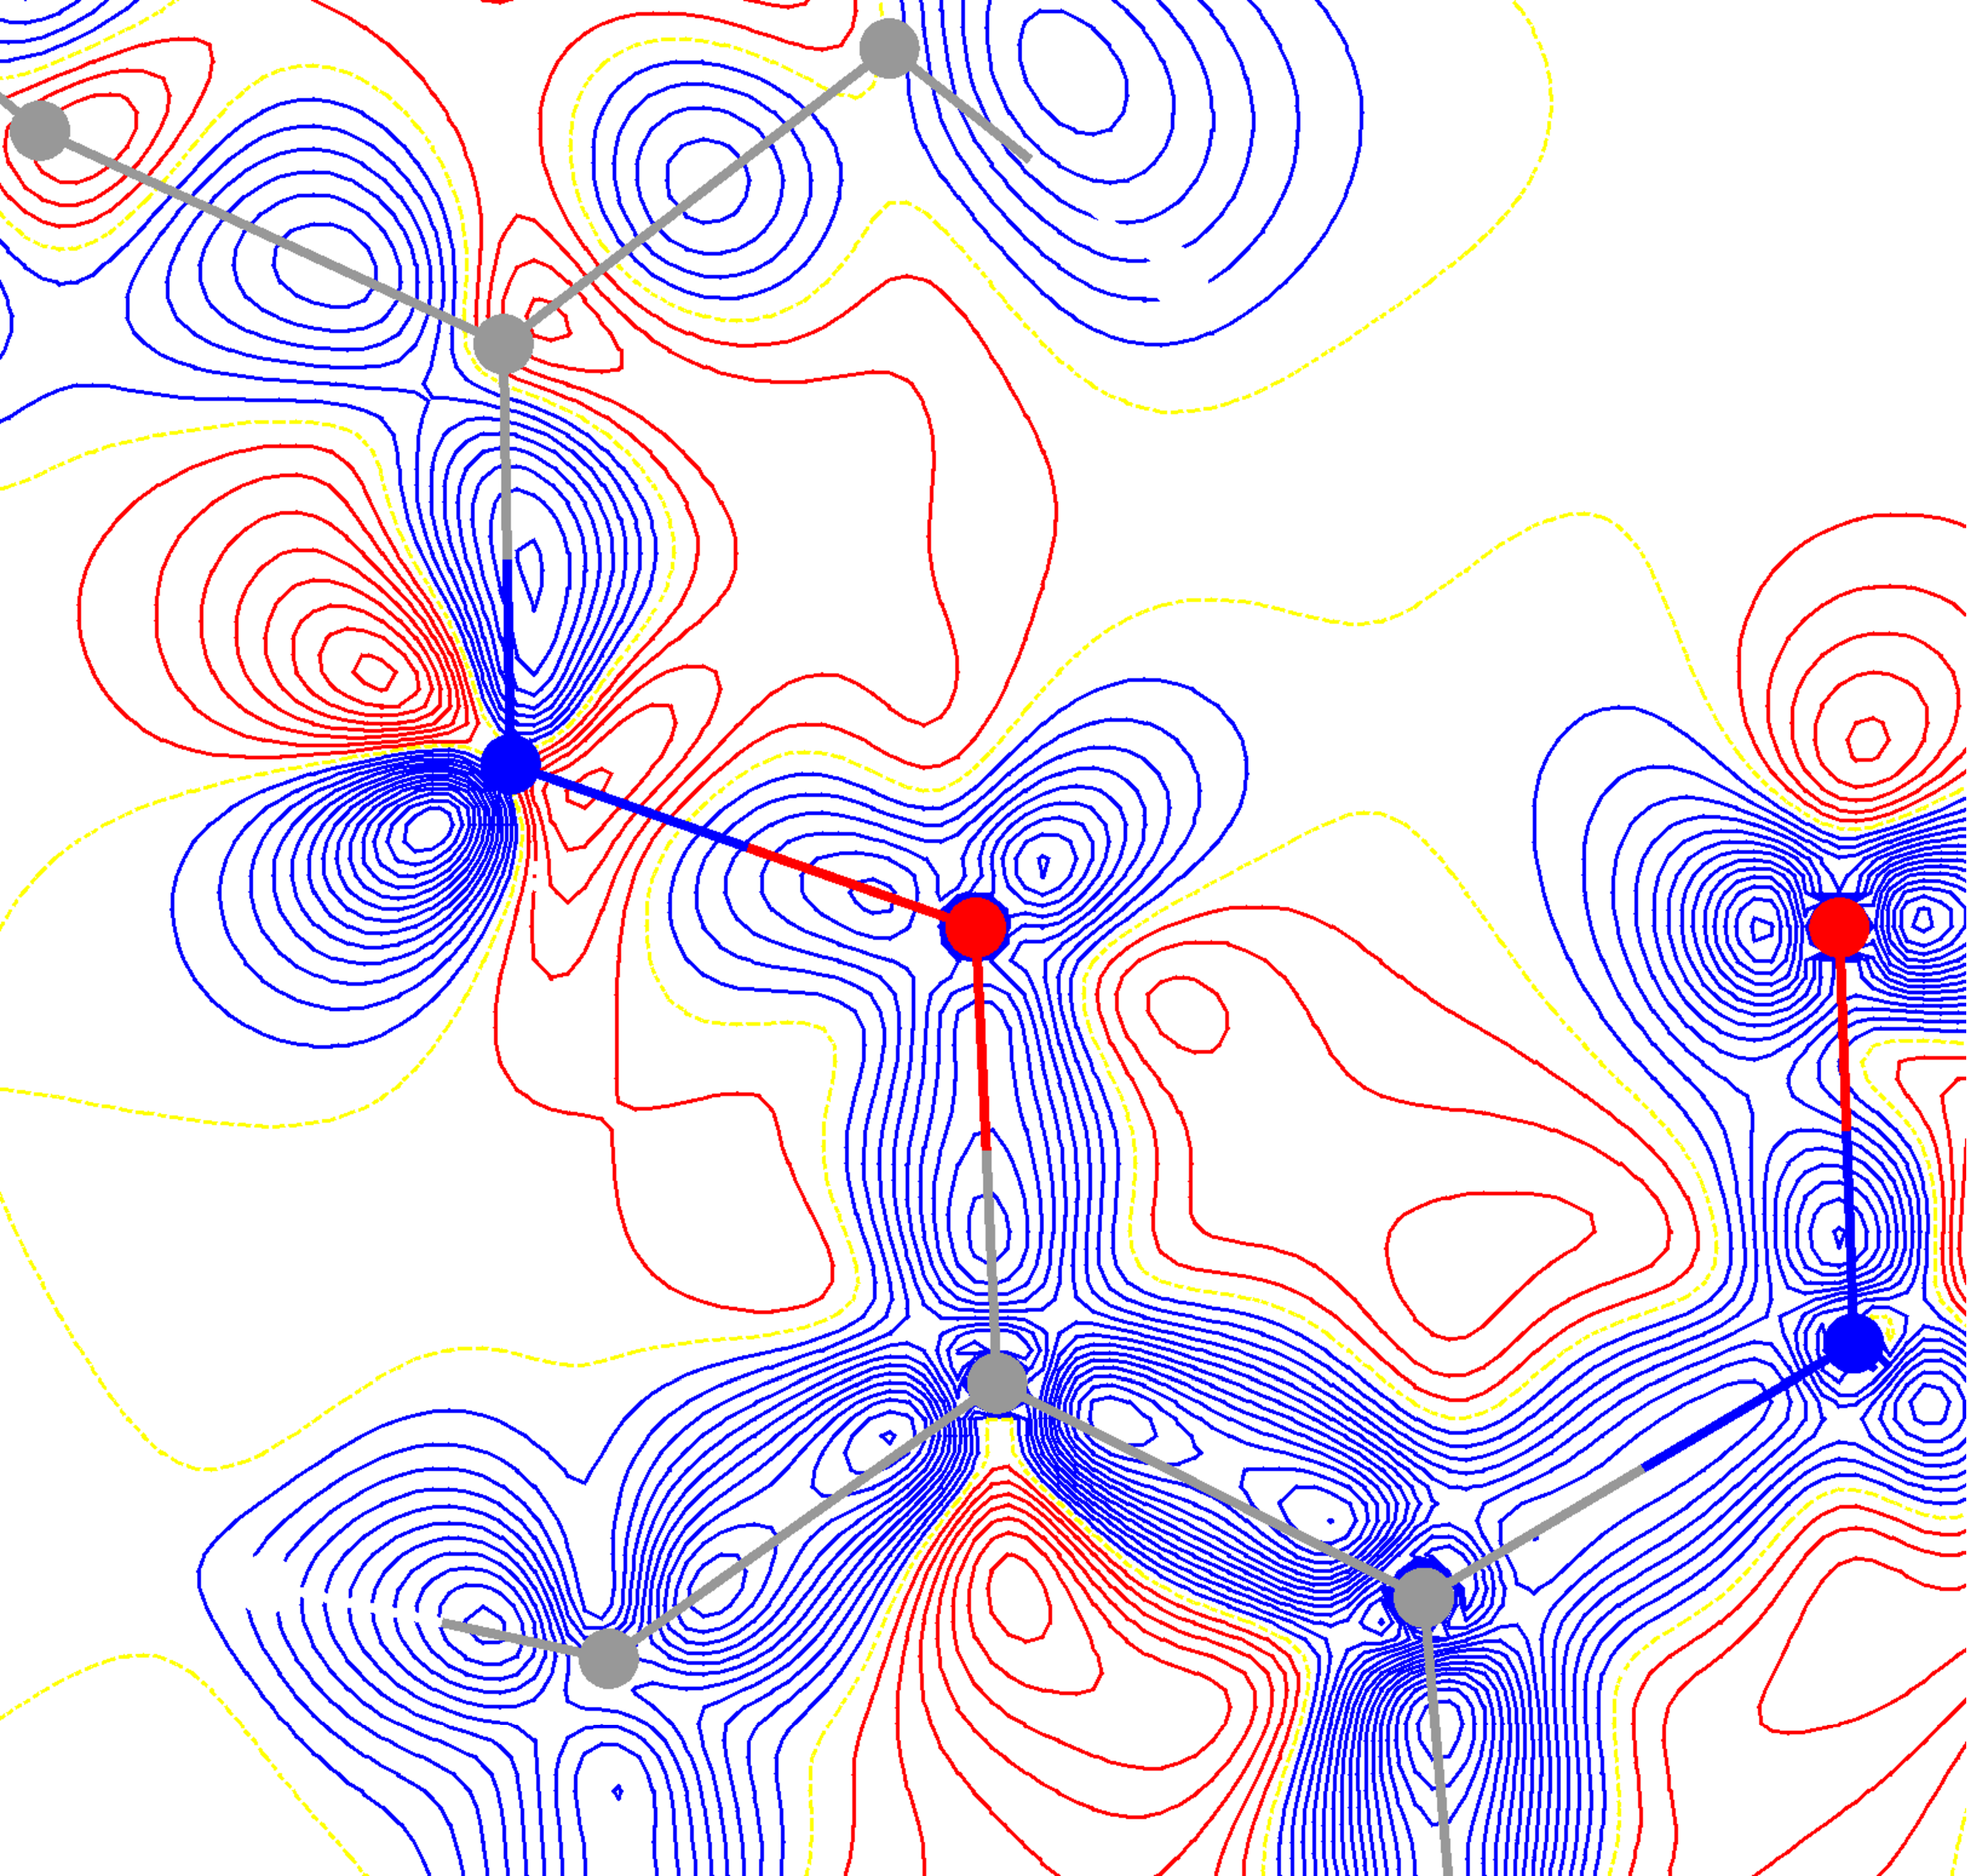
\includegraphics[width=0.45\columnwidth]{Figures/cyclohexanone-oxime-dnp-defdens.pdf}
	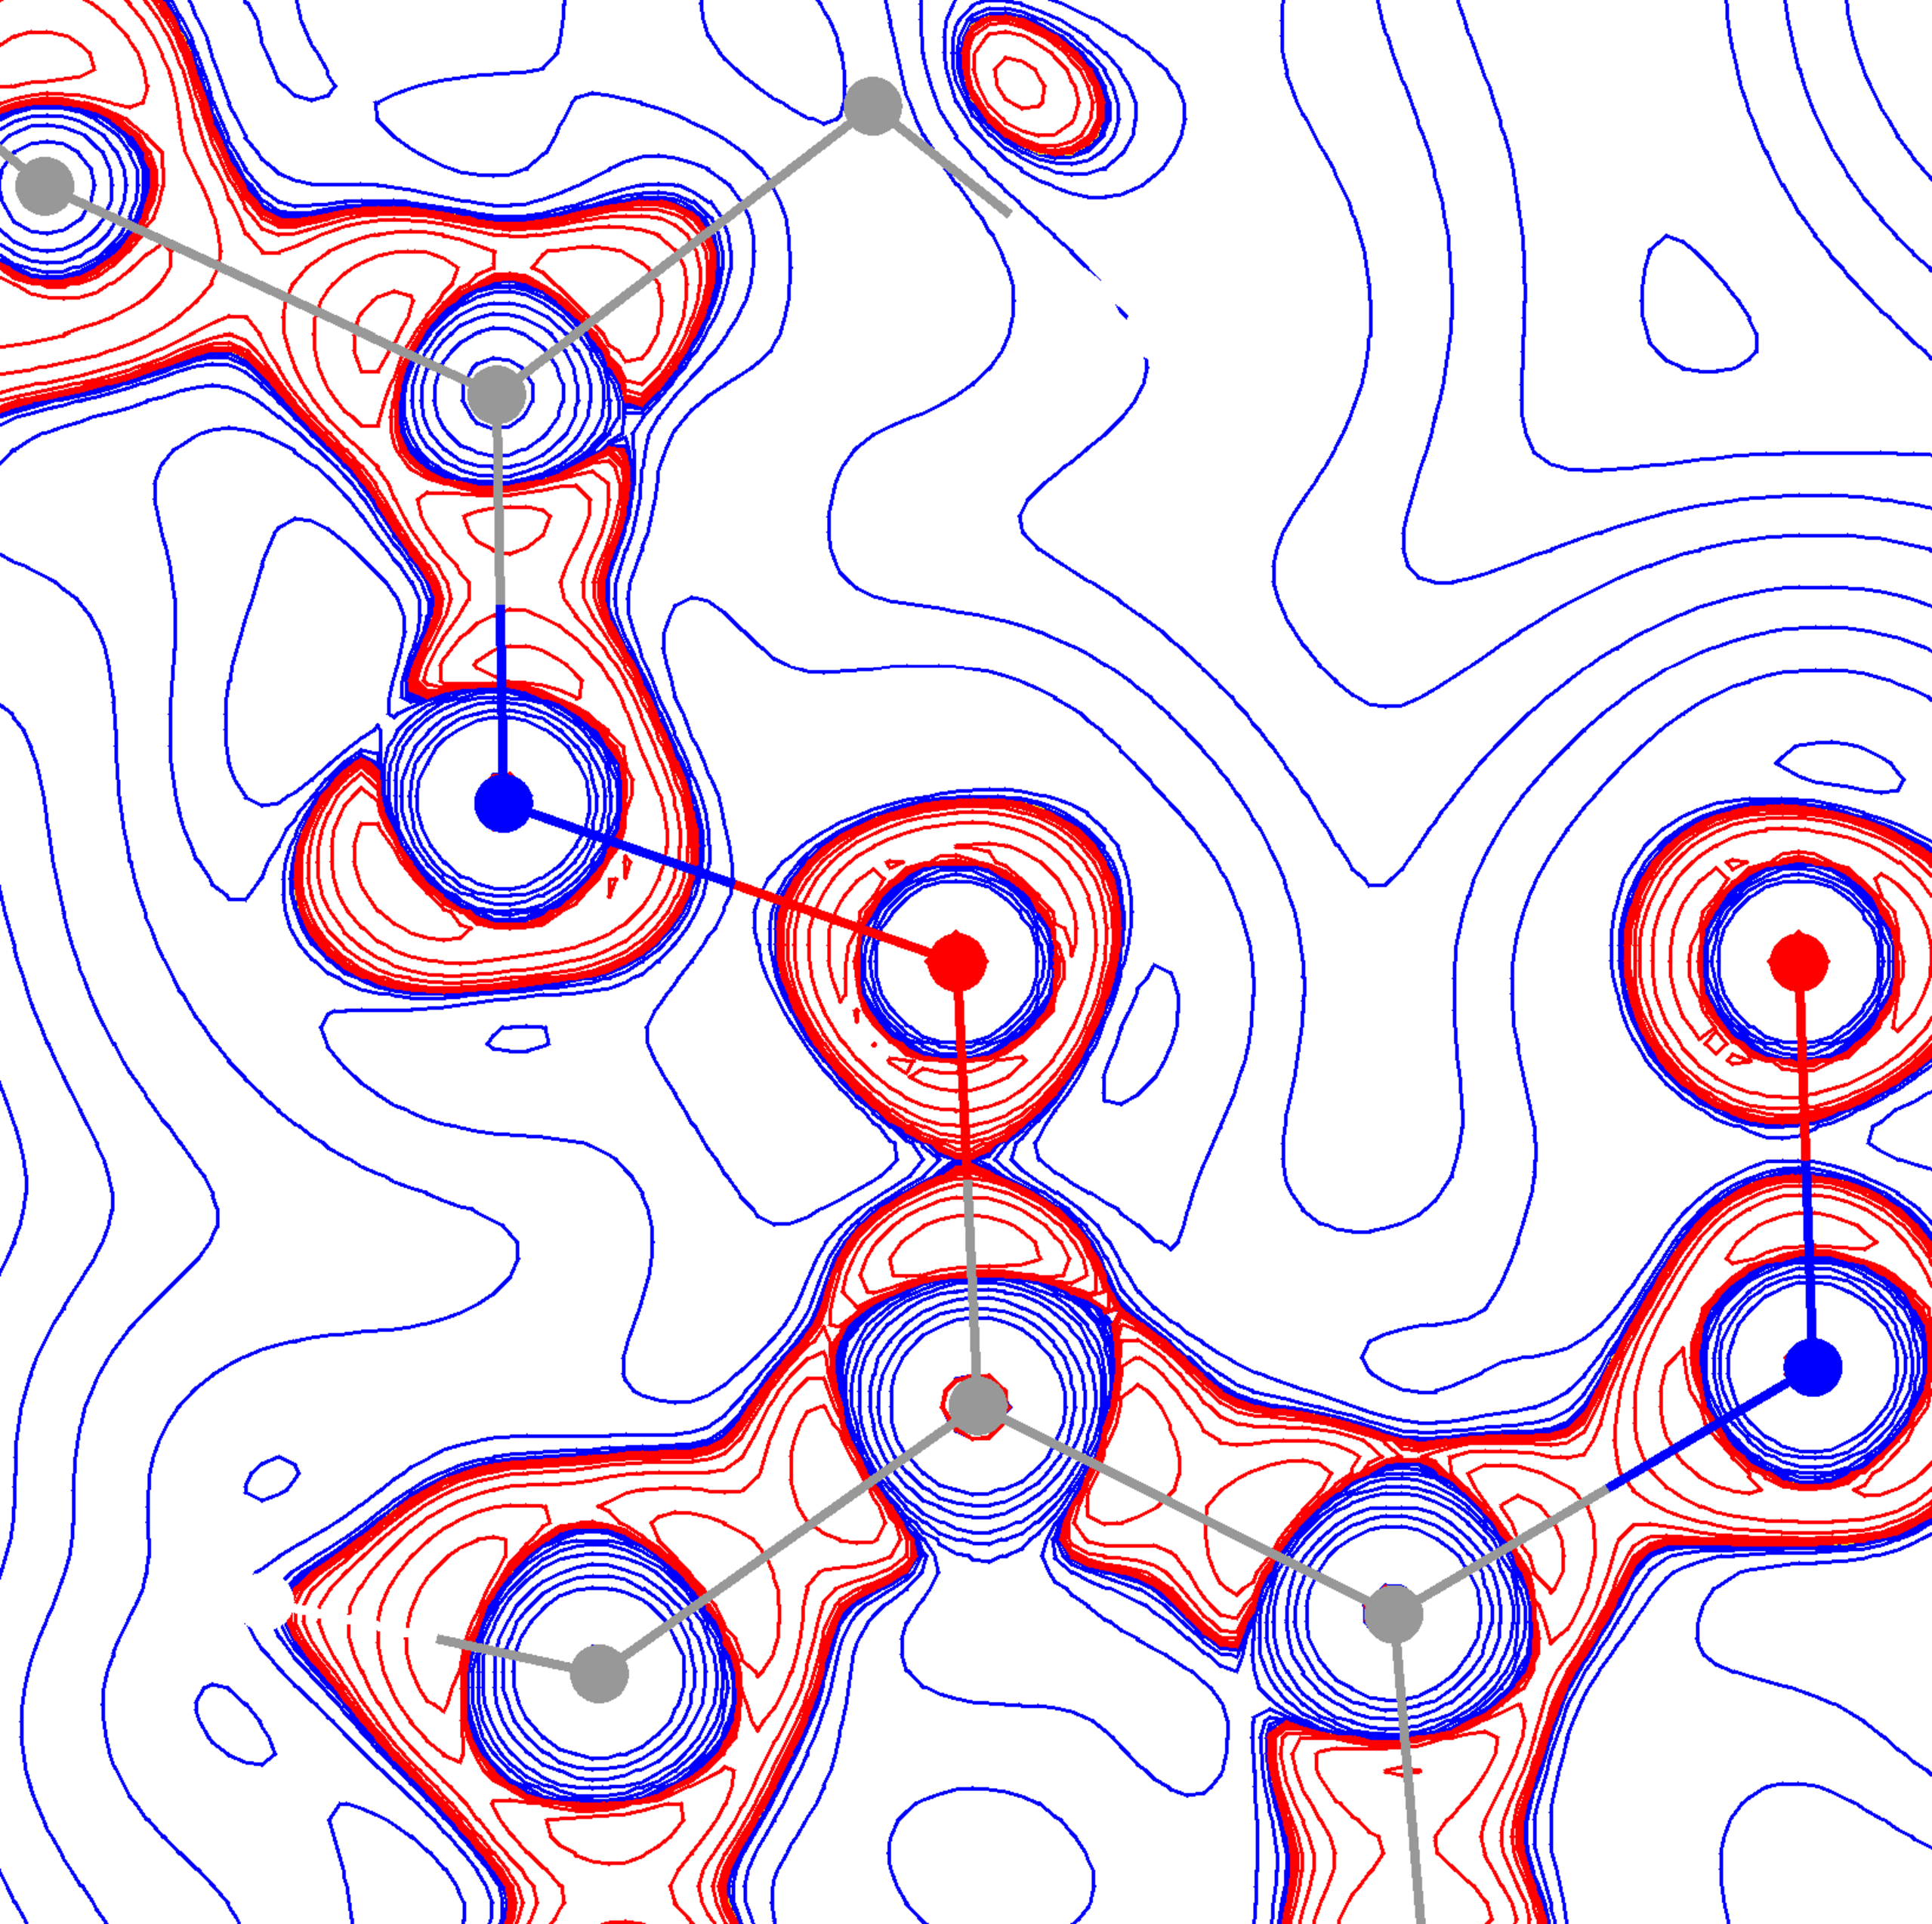
\includegraphics[width=0.45\columnwidth]{Figures/cyclohexanone-oxime-dnp-lapl.pdf}
	\caption{Deformation and Laplacian maps of the experimental electron density for \refcmpd{cyclohexanone-oxime-dnp}. Negative values depicted by red contours, and positive by blue. Above is shown the bond path and bcp in orange.}
	\label{fig:lapl}
\end{figure}

The NCI (non-covalent interaction) index is an extension of QTAIM, which characterises interactions based on the reduced density gradient and the second eigenvalue of the electron density Hessian.\autocite{Johnson2010a}
This can be used to construct informative maps, showing surfaces where non-covalent interactions appear to be occurring.
NCI maps were computed for \cmpd{cyclohexanone-oxime-dnp} and \cmpd{acetone-oxime-dnp} based on the experimental electron density, and these are shown in \cref{fig:NCI}.

\begin{figure}
	\centering
	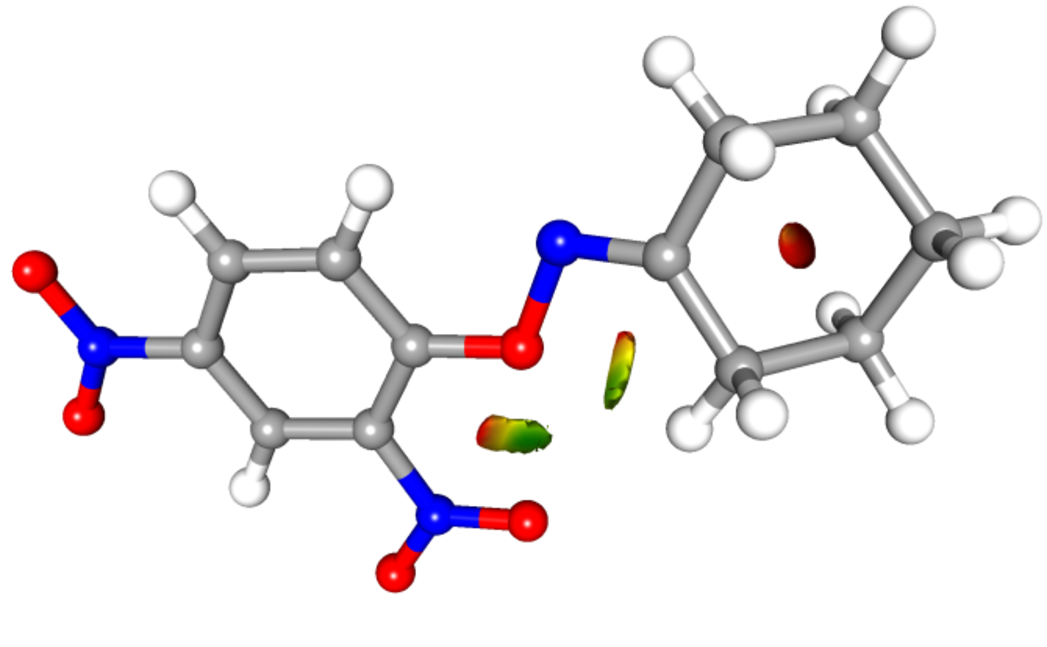
\includegraphics[angle=90,width=0.35\columnwidth]{Figures/cyclohexanone-oxime-dnp-nci.pdf}
	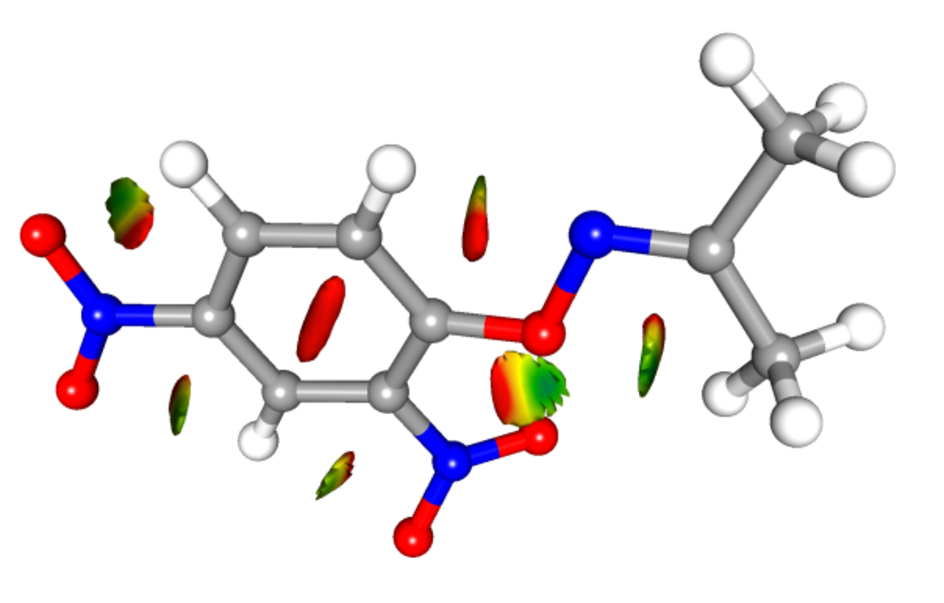
\includegraphics[angle=90,width=0.35\columnwidth]{Figures/acetone-oxime-dnp-nci.pdf}
	\caption{NCI maps for \refcmpd{cyclohexanone-oxime-dnp} and \refcmpd{acetone-oxime-dnp}. Positive values (non-bonding) are shown in red, and negative values (attractive) are shown in blue.}
	\label{fig:NCI}
\end{figure}

To provide further evidence for the interaction, we took advantage of the fact that derivative \cmpd{acetone-oxime-dnp} does not display a Ch-bond, and searched for a $\sigma$-hole in the experimental electron density.
Due to the crowded surroundings of the oxime group, we were unable to visualise the 0.001~a.u. isosurface as would be typical for ESP analysis.
The extension of the oxime bond (therefore, the $\sigma$-hole) was simply not visible.
We instead mapped the electrostatic potential onto intersecting planes through the oxime bond, which clearly showed an positive region along the extension of this bond consistent with a $\sigma$-hole (\cref{fig:acetone-esp}).

\begin{figure}
	\centering
	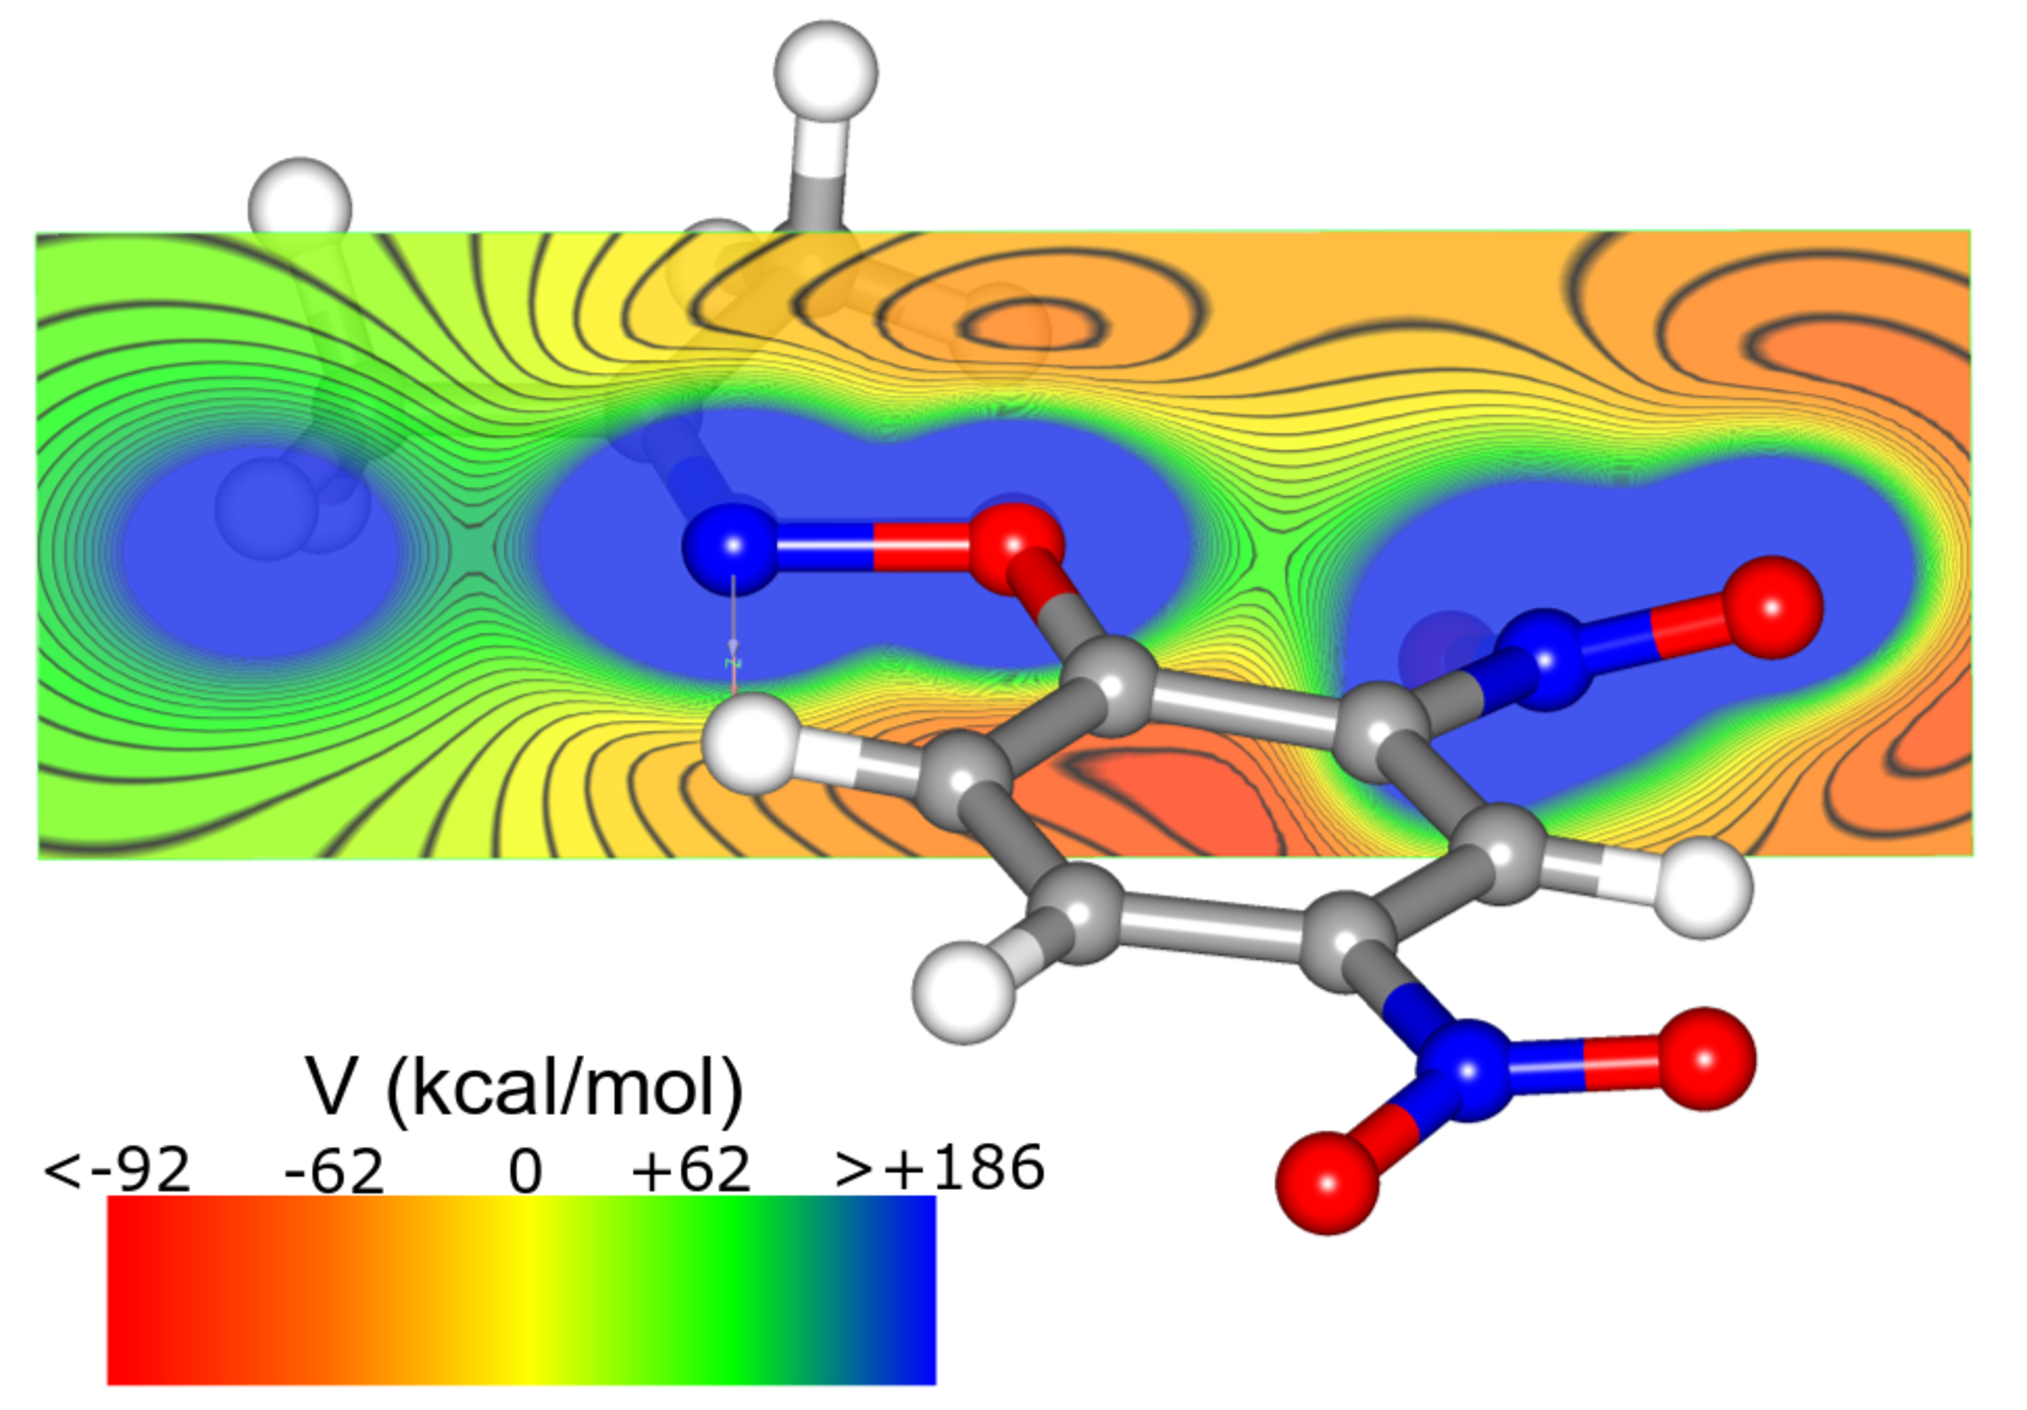
\includegraphics[width=0.6\columnwidth]{Figures/acetone-oxime-dnp-esp.pdf}
	\caption{Electrostatic potential mapped onto a plane through the oxime bond. The $\sigma$-hole is visible as a green (positive ESP) elongation of the nuclear potential towards the nitro group to the right. Note that the oxime nitrogen also displays a $\sigma$-hole to the left.}
	\label{fig:acetone-esp}
\end{figure}

When investigating such weak interactions as these, it is important to consider the limitations of each method of analysis.
For example, the presence of a topological bond path within the QTAIM framework does not necessarily imply the presence of an attractive bonding interaction.
It may simply represent the inevitable consequence of placing two electron clouds in close proximity.\autocite{Spackman1999,Gatti2005,Bader2009,Cerpa2008,Cerpa2009}
However, in this case, the NBO calculations, QTAIM and electrostatic potential analysis of the experimental electron densities are all consistent with the statistically significant lengthening of the oxime \ce{N-O} bond, and all signs point toward a true $\sigma$-hole interaction.

We believe this is the first documented experimental evidence of a $\sigma$-hole interaction at oxygen, and it is remarkable that it occurs in such air- and water-stable molecules as these oximes.
We therefore challenge the consensus that Ch-bonding can only occur at highly activated oxygen atoms, and suggest that there may be implications when considering the reactivity of trace molecules such as peroxides, and nitric and nitrous oxides in biological systems.

\section{Supplementary material}

\subsection{Synthesis}

\subsubsection{Preparation of \emph{O}-(2,4-dinitrophenyl) oximes \refcmpd{cyclohexanone-oxime-dnp,acetone-oxime-dnp}}
Cyclohexanone oxime (556.8~mg, 4.920~mmol) and sodium hydride (60\% in mineral oil, 249.5~mg, 6.237~mmol) were dissolved in anhydrous THF (10~mL) and stirred for 5 minutes. This was then added to a solution of 2,4-dinitro-1-fluorobenzene (950.6~mg, 5.108~mmol) in a further 10~mL anhydrous THF. This was stirred for 1~h at room temperature, then diluted with water (100~mL) and extracted with ethyl acetate (2$\times$30~mL). The combined organic phases were washed with brine (30~mL), dried (\ce{MgSO4}) and evaporated to afford \cmpd{cyclohexanone-oxime-dnp} as a waxy pale yellow solid (895.1~mg, 65\%, m.p. 100.2--100.9\degree~C).

Acetone oxime \cmpd{acetone-oxime-dnp} was isolated as a pale yellow powder, yield 72\%, m.p. 88.5--88.9\degree~C.

Crystals suitable for x-ray diffraction analysis were grown by slow diffusion of pentane into a saturated solution of the compound in dichloromethane.

\subsection{Crystallographic data}

\subsubsection{Crystal data for \texorpdfstring{dimethylcyclohexanone-oxime-dnp}{C14H17N3O5}}
\ce{C14H17N3O5} (\emph{M} = 307.30 g/mol): monoclinic, space group P2\textsubscript{1}/c (no. 14), \emph{a} = 7.17630(10)~\AA , \emph{b} = 28.9373(4)~\AA , \emph{c} = 7.06700(10)\AA , $\beta$ = 92.1860(10)\degree, V = 1466.48(4)~\AA$^3$, \emph{Z} = 4, \emph{T} = 130.15~K, $\mu$(Cu K$\alpha$) = 0.902~mm$^{-1}$, \emph{Dcalc} = 1.392~g/cm$^3$, 10358 reflections measured (12.234\degree $\leq 2\theta \leq$ 158.922\degree), 2902 unique (R\textsubscript{int} = 0.0231, R\textsubscript{sigma} = 0.0149) which were used in all calculations. The final R\textsubscript{1} was 0.0472 (I $> 2\sigma$(I)) and wR\textsubscript{2} was 0.1242 (all data).

\subsubsection{Crystal data for \texorpdfstring{cyclohexanone-oxime-dnp}{C12H13N3O5}}
\ce{C12H13N3O5} (\emph{M} = 279.25 g/mol): monoclinic, space group P2\textsubscript{1} (no. 4), \emph{a} = 6.66740(10)~\AA, \emph{b} = 16.3925(3)~\AA, \emph{c} = 11.6108(2)~\AA, $\beta$ = 101.0310(10)\degree, V = 1245.56(4)~\AA$^3$, \emph{Z} = 4.00, \emph{Z'} = 2.00, \emph{T} = 100(1) K, $\mu$(Mo K$\alpha$) = 0.118~mm$^{-1}$, \emph{Dcalc} = 1.489~g/cm$^3$, 51580 reflections measured (7.016\degree $\leq 2\theta \leq$ 102.638\degree), 25111 unique (R\textsubscript{int} = 0.0214, R\textsubscript{sigma} = 0.0317) which were used in all calculations. The final R\textsubscript{1} was 0.0409 (I $> 2\sigma$(I)) and wR\textsubscript{2} was 0.1153 (all data). Flack parameter = $0.32(14)$.

\subsubsection{Crystal data for \texorpdfstring{acetone-oxime-dnp}{C9H9N3O5}}
\ce{C9H9N3O5} (\emph{M} = 239.175 g/mol): orthorhombic, space group P2\textsubscript{1}2\textsubscript{1}2\textsubscript{1} (no. 19), \emph{a} = 5.49110(10)~\AA, \emph{b} = 10.5173(2)~\AA, \emph{c} = 18.2619(3)~\AA, \emph{V} = 1054.65(3)~\AA$^3$, \emph{Z} = 4, \emph{T} = 100.00(10)~K, $\mu$(Mo K$\alpha$) = 0.125~mm$^{-1}$, \emph{Dcalc} = 1.506~g/cm$^3$, 24292 reflections measured (5.908\degree $\leq 2\theta \leq$ 102.41\degree), 10696 unique (R\textsubscript{int} = 0.0224, R\textsubscript{sigma} = 0.0326) which were used in all calculations. The final R\textsubscript{1} was 0.0378 (I $> 2\sigma$(I)) and wR\textsubscript{2} was 0.1032 (all data). Flack parameter = $-0.02(19)$.

\printbibliography
\end{refsection}

